\clearpage
\section{Kramers-Kronig Transceiver  with Stokes PolDemux}

\begin{tcolorbox}	
\begin{tabular}{p{2.75cm} p{0.2cm} p{10.5cm}} 	
\textbf{Student Name}  &:& Romil Patel\\
\textbf{Starting Date} &:& August 16, 2017\\
\textbf{Goal}          &:& Develop a simplified structure (low cost) for a coherent transceiver, that can be used in coherent PON, inter-data center connections, or metropolitan networks (optical path lengths < 100 km). We are going to explore a Kramers-Kronig transceiver with Stokes based PolDemux.\\
\textbf{Directory} 	   &:&LinkPlanner\textbackslash doc\textbackslash tex\textbackslash sdf\textbackslash simplified\_coherent\_receiver 
\end{tabular}
\end{tcolorbox}

Coherent optical transmission schemes are spectrally efficient since they allow the encoding of information in both quadrature of sinusoid signal. However, the cost of coherent receiver becomes a major obstacle in the case of short-reach links applications like PON, inter-data-center communications and metropolitan network. In order to make the transceiver applicable in short-reach links, an architecture has been proposed which combines the advantages of coherent transmission and cost effectiveness of direct detection. The working principle of the proposed transceiver is based on the Kramers-Kronig (KK) relationship. The KK transceiver scheme allows digital compensation of propagation impairment because both amplitude and phase of the electrical field can be retrieved at the receiver. 
\subsection{Theoretical Analysis}
The Kramers-Kronig relations are bidirectional mathematical relations, connecting the real and imaginary parts of any complex function that is analytic in the upper half-plane. For instance, a signal $x(t)=x_r(t) + i x_i(t)$ satisfies the Kramers-Kronig relationship if,
\begin{equation*}
\begin{split}
x_{r}(t) &=-\frac{1}{\pi} p.v. \int_{-\infty}^{\infty} \frac{x_{i}(t')}{t-t'} dt' \\ \\
x_{i}(t) &=\frac{1}{\pi} p.v. \int_{-\infty}^{\infty} \frac{x_{r}(t')}{t-t'} dt' \\
\end{split}
\label{KK}
\end{equation*}
This relationship imposes that the real and the imaginary parts of the signal are related to each other though Hilbert transform. Therefore, if we have the real part of the signal then the imaginary part can be calculated by its Hilbert transform. \\For a signal that satisfies the Kramers-Kronig relationship, the real and imaginary part can be obtained only from the module. The following questions would give a comprehensive overview of Kramers-Kroning relation and the detailed mathematical calculation which depicts how phase can be extracted from the amplitude information.

\subsubsection{1. What is Hilbert transform?}
If we consider a filter $H(\omega)$, described in Figure \ref{Hilbert_Transformer}, that has a unity magnitude response for all frequencies and the phase response is $-\pi/2$ for all positive frequencies and $\pi/2$ for negative frequencies. The transfer function of this filter is given by
\begin{equation}
\begin{split}
H(\omega)=-isgn(\omega)
\end{split}
\label{}
\end{equation}
\begin{figure}[h]
	\centering
	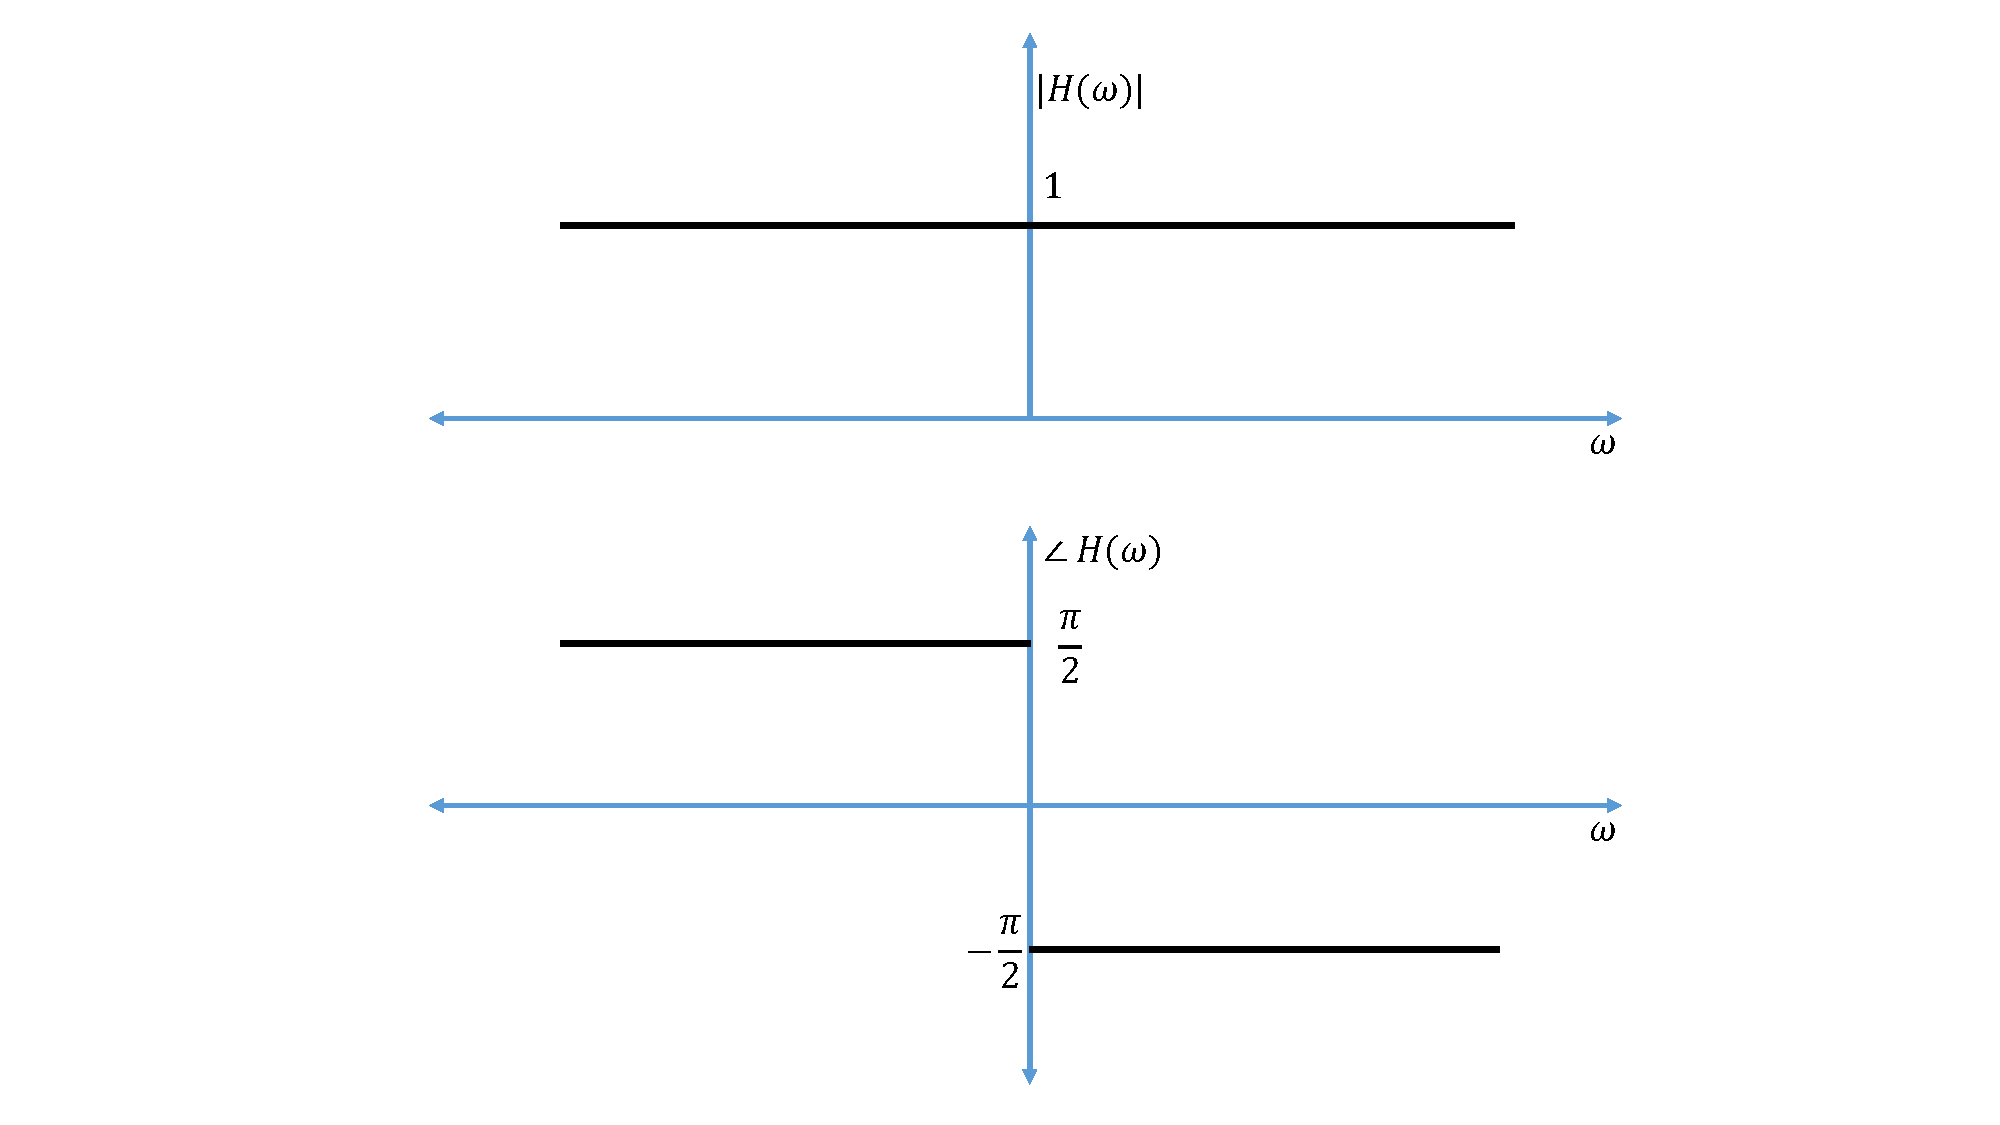
\includegraphics[width=1.0\textwidth, height=8cm]{./sdf/simplified_coherent_receiver/figures/HT.pdf}
	\caption{Magnitude and phase of Hilbert transform filter}\label{Hilbert_Transformer}
\end{figure}
\\
\\
\\
The inpulse response of this filter can be given as,

\begin{figure}[h]
	\centering
	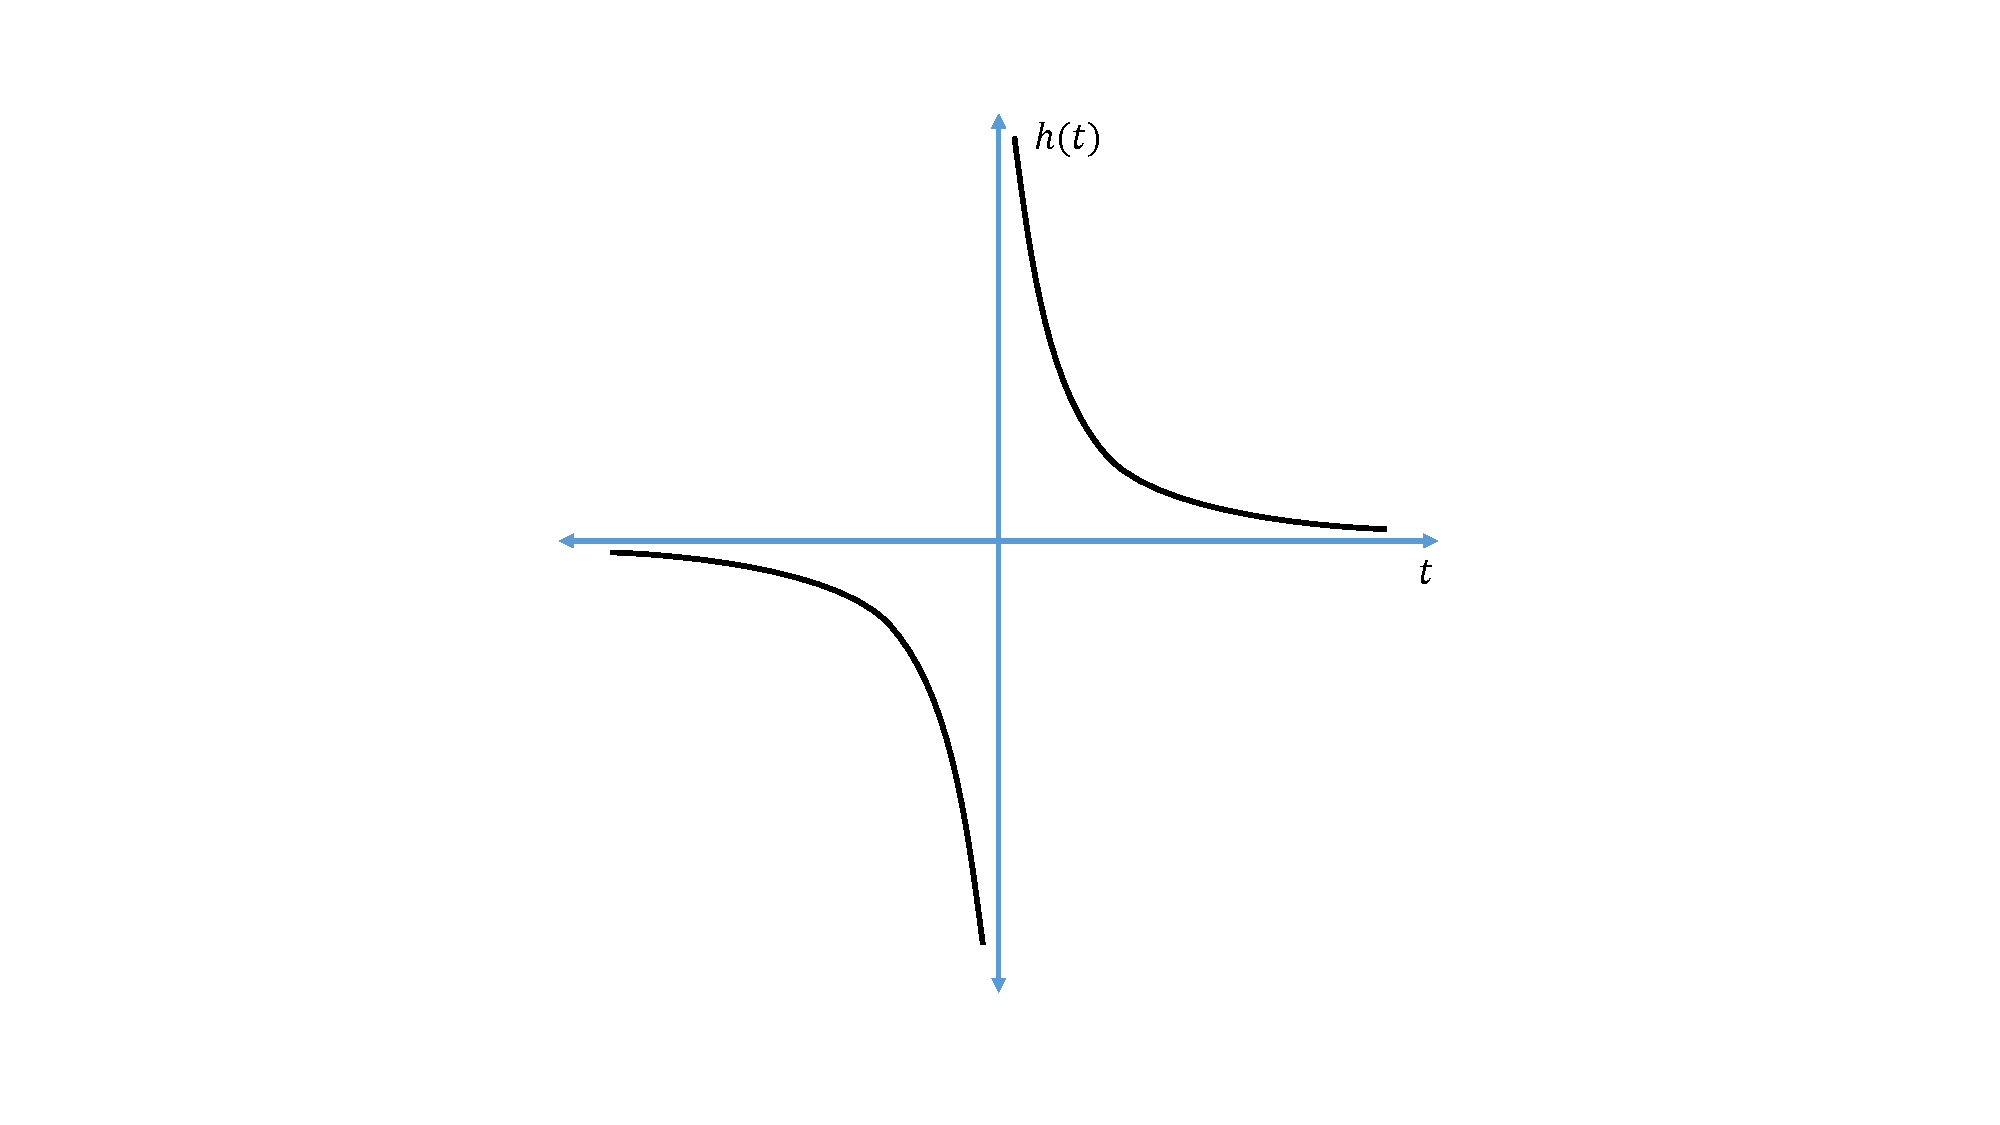
\includegraphics[width=1.0\textwidth, height=8cm]{./sdf/simplified_coherent_receiver/figures/Impulse_Response.pdf}
	\caption{Impulse response $h(t)$ of Hilbert transform filter}\label{Impulse_Response}
\end{figure}

\begin{equation}
\begin{split}
h(t)&=\mathcal{F}^{-1}[H(i\omega)]\\
&=-i\mathcal{F}^{-1}[sgn(\omega)]\\
&=-i\bigg(\frac{i}{\pi t}\bigg)\\
&=\frac{1}{\pi t}
\end{split}
\label{}
\end{equation}
When this filter driven by an arbitrary signal $s(t)$, the filter produces the output as,
\begin{equation}
\begin{split}
\hat{s}(t)&=s(t) * h(t)\\
&=\int_{-\infty}^{\infty} \dfrac{s(u)}{\pi(t-u)}du\\
\end{split}
\label{}
\end{equation}
The function $\hat{s}(t)$ is called the Hilbert transform if $s(t)$. Note that
\begin{equation}
\begin{split}
\mathcal{F}[\hat{s}(t)]=H(\omega)S(\omega)=-isgn(\omega)S(\omega)
\end{split}
\label{}
\end{equation}
In conclusion, if we convolve any time domain signal with $\frac{1}{\pi t}$ then it will give us Hilbert transformed signal in time domain. Similarly, from the convolution property of the Fourier transform, if we multiply $-isgn(\omega)$ with any frequency domain signal $S(\omega)$ then it'll give us Hilbert transformed signal in frequency domain.

\subsubsection{2. What is analytical signal?}
An analytic signal is a complex-valued signal that has no negative frequency components, and its real and imaginary parts are related to each other by the Hilbert transform.
\begin{equation}
s_a(t)=s(t)+i\hat{s}(t)
\label{Analytical signal}
\end{equation}
where, $s_a(t)$ is an analytical signal and $\hat{s}(t)$ is the Hilbert transform of the signal ${s}(t)$. Such analytical signal can be used to generate Single Sideband Signal (SSB) signal.

\subsubsection{3. What is a SSB signal and how it can be generated?}
By definition, the SSB is the signal which contains either upper sideband or lower sideband and hence it reduces the spectral occupancy by half. \\
This section will represent the brief idea of generating SSB signal using Hilbert transform method. To understand this, we may express signal $s(t)$ as a summation of the two complex-valued functions.
\begin{equation}
\begin{split}
s(t)&=\dfrac{1}{2}[s(t)+i\hat{s}(t)]+\dfrac{1}{2}[s(t)-i\hat{s}(t)]\\
\end{split}
\label{}
\end{equation}
From Equation \ref{Analytical signal},
\begin{equation}
\begin{split}
	s(t)&=s_a(t)+i{s_a^*}(t)
\end{split}
\label{}
\end{equation}
%where, the term $\dfrac{1}{2}[s(t)+i\hat{s}(t)]$ is the analytical representation of the signal $s(t)$ (from Equation \ref{Analytical signal}). Another term represents the complex conjugate $\dfrac{1}{2}[s(t)-i\hat{s}(t)]$ of this analytical signal.
Such representation of ${s_a}(t)$ and ${s_a^*}(t)$ divide the signal into non-negative frequency component and non-positive frequency component respectively. Considering only non-negative frequency ${s_a}(t)$ part, we can write it as
\begin{equation}
\dfrac{1}{2}{S_a}(f) = \begin{cases}
S(f) &\text{for $f>0$}\\
0    &\text{for $f<0$}\\
\end{cases}
\end{equation}
where ${S_a}(f)$ and ${S}(f)$ are the Fourier transform of ${t_a}(t)$ and ${s}(t)$ respectively. The frequency translated version of ${S_a}(f-f_0)$ contains only one side (positive) of ${S}(f)$ and hence it is called single sideband signal ${s_{ssb}}(t)$,
\begin{equation}
{F}^{-1}\{S_a(f-f_0)\}={s_a}(t) e^{i2\pi f_0 t}={s_{ssb}}(t)+i{\hat{s}_{ssb}(t)}
\end{equation}
Therefore, from the Euler's formula,
\begin{equation}
\begin{split}
{s}_{ssb}(t)&=Re\{s_a(t)  e^{i2\pi f_0 t}\}\\
&=Re\{[s(t)+i\hat{s}(t)] [cos(2\pi f_0t)+isin(2\pi f_0t)]\}\\
&=s(t)cos(2\pi f_0t)-\hat{s}(t)sin(2\pi f_0t)
\end{split}
\label{USB_SSB}
\end{equation}
This Equation \ref{USB_SSB} displays the mathematical modeling of the upper sideband SSB signal. Similarly, we can generate lower sideband SSB signal by,
\begin{equation}
{s}_{ssb}(t)=s(t)cos(2\pi f_0t)+\hat{s}(t)sin(2\pi f_0t)
\label{LSB_SSB}
\end{equation}

\subsubsection{4. What is minimum phase signal?}
A necessary and sufficient condition for a complex signal $A(t)$ to be minimum phase is that the curve described in a complex plane by $A(t)$ when $t\rightarrow -\infty$ to $t\rightarrow \infty$ \textbf{does not encircle the origin}. A minimum-phase signal has an useful property that the natural logarithm of the magnitude of the frequency response is related to the phase angle of the frequency response by the Hilbert transform.\\
For instance, if we consider a complex data-carrying signal whose spectrum is contained between $-B/2$ and $B/2$, and consider a SSB signal of the form,
\begin{equation}
x(t)=A + A_{s}(t)exp(-i\pi Bt)
\label{}
\end{equation}
where A is a constant. Here, $x(t)$ is minimum phase if and only if the winding number of its trajectory into complex plane is zero. The condition $|A|>|A_{s}(t)|$ is sufficient for guaranteeing minimum phase property [3]. 

\subsubsection{5. How we can use these signals and profit from them?}
This section represents the justification that why we need to use these signals into our proposed transceiver system.\\ \\
\textbf{Analytical Signal:}\\
If we denote an analytic signal $A_s(t)$ as, 
\begin{equation}
A_s(t)=A_{s,r}(t)+iA_{s,i}(t)
\label{Eq:5.31}
\end{equation}
then in the equation \ref{Eq:5.31}, the real and imaginary parts $A_{s,r}(t)$ and $A_{s,i}(t)$ are related through the Kramers-Kronig relation with each other. An intuitive way to analyze the relation is based on expressing its Fourier transform $A_s(\omega)$ as follows,
\begin{equation}
A_s(\omega)=\dfrac{1}{2}[1+sgn(\omega)]A_s(\omega)
\label{Eq:A}
\end{equation}
The equation \ref{Eq:A} follows the SSB signal condition $A_s(\omega)=0$ for $\omega<0$. Further, simplification0n of the signal can be summarized as follows:
\begin{equation}
\begin{split}
A_s(\omega)&=\dfrac{1}{2}[1+sgn(\omega)]A_s(\omega)\\
&=\dfrac{1}{2}A_s(\omega)+\dfrac{1}{2}sgn(\omega)A_s(\omega)
\end{split}
\label{Eq:B}
\end{equation}
Taking inverse Fourier transform of the equation \ref{Eq:B},
\begin{equation}
\begin{split}
{A_s}(t)&=IFT\{A_s(\omega)\}\\
&=\dfrac{1}{2}{A_s}(t)+\underline{\dfrac{1}{2}[IFT\{sgn(\omega)\} \circledast {A_s}(t)]}
\end{split}
\label{Eq:C}
\end{equation}
The underlined term in Equation \ref{Eq:C} displays that multiplication in frequency domain converted into the convolution in the time domain. Further, IFT of the function $sgn(\omega)$ given as $(-i/\pi t)$. As a consequences, we can further simplify our equation as,
\begin{equation}
\begin{split}
{A_s}(t)&=\dfrac{1}{2}{A_s}(t)+\frac{1}{2}\bigg[\frac{i}{\pi t} \circledast {A_s}(t) \bigg]\\
\frac{{A_s}(t)}{2} &=\frac{1}{2}\bigg[\frac{i}{\pi t} \circledast {A_s}(t) \bigg]\\
{A_s}(t) &=i\bigg[\frac{1}{\pi t} \circledast {A_s}(t) \bigg]\\
{A_s}(t) &=\frac{i}{\pi} p.v. \int_{-\infty}^{\infty} \frac{A_s(t')}{t-t'} dt' 
\end{split}
\label{Eq:D}
\end{equation}
Using Equation \ref{Eq:5.31} into Equation \ref{Eq:D},
\begin{equation}
\begin{split}
A_{s,r}(t)+iA_{s,i}(t) &=\frac{i}{\pi} p.v. \int_{-\infty}^{\infty} \frac{A_s(t')}{t-t'} dt' 
\end{split}
\label{Eq:5.36}
\end{equation}
Therefore,
\begin{equation}
\begin{split}
A_{s,r}(t)+iA_{s,i}(t) &=\frac{i}{\pi} p.v. \int_{-\infty}^{\infty} \frac{A_{s,r}(t')+iA_{s,r}(t')}{t-t'} dt' \\
A_{s,r}(t)+iA_{s,i}(t)&=-\frac{1}{\pi} p.v. \int_{-\infty}^{\infty} \frac{A_{s,i}(t')}{t-t'} dt' + \frac{i}{\pi} p.v. \int_{-\infty}^{\infty} \frac{A_{s,r}(t')}{t-t'} dt'
\end{split}
\label{Eq:5.37}
\end{equation}
which leads to,
\begin{equation}
\begin{split}
A_{s,r}(t) &=-\frac{1}{\pi} p.v. \int_{-\infty}^{\infty} \frac{A_{s,i}(t')}{t-t'} dt' \\
A_{s,i}(t) &=\frac{1}{\pi} p.v. \int_{-\infty}^{\infty} \frac{A_{s,r}(t')}{t-t'} dt' \\
\end{split}
\label{Eq:5.38}
\end{equation}\\
\textbf{Minimum Phase signal:}\\
Given function $A(t)=A_{s}(t)+\bar{A}$ never encircles the origin for $t\in(-\infty,\infty)$. if we define,
\begin{equation}
G(t)=log\bigg[\dfrac{A(t)}{\bar{A}}\bigg]\\
\label{Eq:A1}
\end{equation} 
then $G(\omega)$, the spectrum of $G(t)$, is such that $G(\omega)=0$ for $\omega<0$. Under the hypothesis stated by Equation \ref{Eq:5.36}, we can write $G(t)$ as,
\begin{equation}
\begin{split}
G(t) &=\frac{i}{\pi} p.v. \int_{-\infty}^{\infty} \frac{G(t')}{t-t'} dt' 
\end{split}
\label{Eq:B1}
\end{equation}
From the equations \ref{Eq:A1} and \ref{Eq:B1},
\begin{equation}
\begin{split}
log|A(t)|-log|\bar{A}|+i[\phi(t)-\bar{\phi}] &=\frac{i}{\pi} p.v. \int_{-\infty}^{\infty} \frac{log|A(t)|-log|\bar{A}|}{t-t'} dt' + \frac{1}{\pi} p.v. \int_{-\infty}^{\infty} \frac{\phi(t)-\bar{\phi}}{t-t'} dt' 
\end{split}
\label{Eq:C1}
\end{equation}
Comparing Imaginary part of Equation \ref{Eq:C1},
\begin{equation}
\begin{split}
\phi(t)-\bar{\phi} &= + \frac{1}{\pi} p.v. \int_{-\infty}^{\infty} \frac{log|A(t)|-log|\bar{A}|}{t-t'} dt'\\
\end{split}
\label{Eq:D1}
\end{equation}
In equation \ref{Eq:D1}, $\frac{1}{\pi} p.v. \int_{-\infty}^{\infty} \frac{log|\bar{A}|}{t-t'} dt'=0$ which leads to,
\begin{equation}.
\begin{split}
\phi(t) &= \bar{\phi} + \frac{1}{\pi} p.v. \int_{-\infty}^{\infty} \frac{log|A(t)|}{t-t'} dt'\\
\phi(t) &= \bar{\phi} + \frac{1}{2\pi} p.v. \int_{-\infty}^{\infty} \frac{log|A(t)|^2}{t-t'} dt'\\
\end{split}
\label{Eq:E1}
\end{equation}
\newpage
\subsection{Simulation Analysis}
\subsubsection{Transmitter setup}
\begin{center}
\begin{figure}[h]
	\centering
	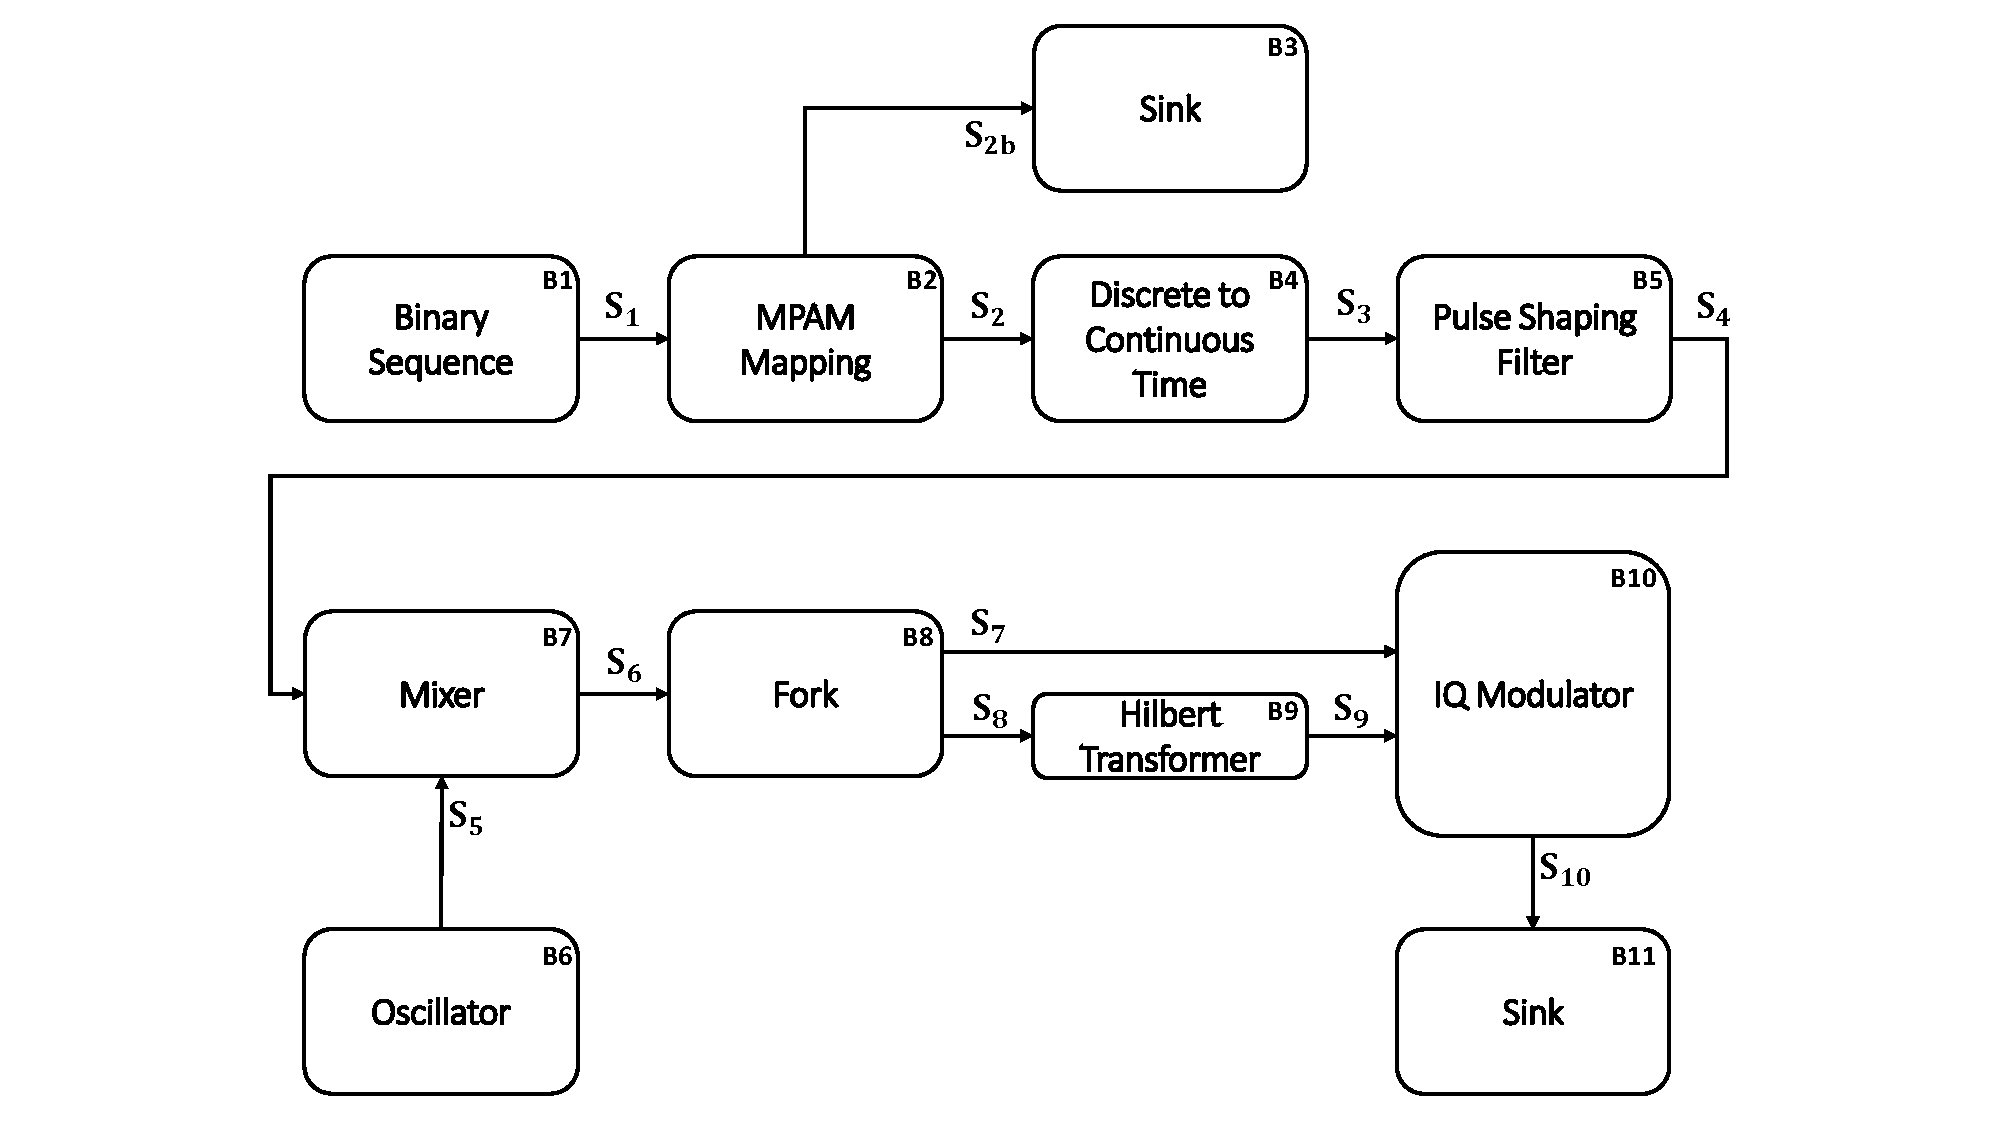
\includegraphics[width=1\textwidth, height=9cm]{./sdf/simplified_coherent_receiver/figures/Simulation_setup_Tx.pdf}
	\caption{Transmitter simulation setup}\label{Simulation_setup_Tx}
\end{figure}
\end{center}
\subsubsection{System input parameters:}
\begin{center}
	\begin{tabular}{ |p{5cm}||p{4.5cm}|p{4.5cm}|  }
		\hline
		%\multicolumn{3}{|c|}{\textbf{System Input Parameters }} \\
		%\hline
		\textbf{Parameter} &  \textbf{Default Value} & \textbf{Description}\\
		\hline
		sourceMode    & PseudoRandom &\\
		\hline
		patternLength & 5      & \\
		\hline
		bitPeriod     & 1/1.25e9 & \\
		\hline
		iqAmplitudes  &\{\{0,0\},\{1,0\},\{2,0\},\{3,0\}\} &\\
		\hline
		numberOfBits  &   1000 & \\
		\hline
		numberOfSamplesPerSymbol& 16  &\\
		\hline
		rollOffFactor & 0.3    & \\
		\hline
		impulseResponseTimeLength&16&\\
		\hline
		rfFrequency& 1.25e9 &\\
		\hline
		outputOpticalPower&1e-3&\\
		\hline
		rfAmplitude{ 1.0 }& 1.0 &\\
		\hline
		rfInitialPhase & 0.0 &\\
		\hline
		outputOpticalWavelength & 1550e-9 &\\
		\hline
		opticalPower & 1e-3 &\\
		\hline
%		outputOpticalWavelength&1550e-9&\\
%		\hline
	\end{tabular}
\end{center}
\vspace{0cm}
\subsubsection{Transmitter setup description:}
\begin{center}
	\begin{tabular}{ |p{6cm}||p{5.5cm}|p{2.5cm}|   }
		\hline
		\multicolumn{3}{|c|}{\textbf{Header Files}} \\
		\hline
		\textbf{File name} & \textbf{Comments}&\textbf{Code Status}\\
		\hline
		binary\_source.h    				&  	Integrated	&\checkmark\\
		\hline
		m\_qam\_mapper.h 					&Integrated \hspace{5mm} NEW! &\checkmark\\
		\hline
		discrete\_to\_continuous\_time.h    &  Integrated		&\checkmark\\
		\hline
		pulse\_shaper.h 					& 	Integrated	&\checkmark\\
		\hline
		RF\_Oscillator.h					&Integrated \hspace{5mm} NEW! &\checkmark\\
		\hline
		mixer.h		 						&Integrated \hspace{5mm} NEW! &\checkmark\\
		\hline
		fork.h								&Integrated \hspace{5mm} NEW! &\checkmark\\
		\hline
		hilbert\_transform.h				&Integrated \hspace{5mm} NEW! &\checkmark\\
		\hline
		iq\_modulator.h						&  		&\checkmark\\
		\hline
		sink.h								&  Integrated	&\checkmark\\
		\hline
		netxpto.h							&  Integrated		&\checkmark\\
		\hline
	\end{tabular}
\end{center}
\vspace{0.4cm}
\begin{center}
	\begin{tabular}{ |p{6cm}||p{5.5cm}|p{2.5cm}|   }
		\hline
		\multicolumn{3}{|c|}{\textbf{Source Files}} \\
		\hline
		\textbf{File name} & \textbf{Comments}&\textbf{Code Status}\\
		\hline
		binary\_source.cpp    				& Integrated &\checkmark\\
		\hline
		m\_qam\_mapper.cpp 					& Integrated \hspace{5mm} NEW! &\checkmark\\
		\hline
		discrete\_to\_continuous\_time.cpp  & Integrated &\checkmark\\
		\hline
		pulse\_shaper.cpp 					& Integrated &\checkmark\\
		\hline
		RF\_Oscillator.cpp					& Integrated \hspace{5mm} NEW! &\checkmark\\
		\hline
		mixer.cpp		 					& Integrated \hspace{5mm} NEW! &\checkmark\\
		\hline
		fork.cpp							& Integrated \hspace{5mm} NEW! &\checkmark\\
		\hline
		hilbert\_transform.cpp				& Integrated \hspace{5mm} NEW! &\checkmark\\
		\hline
		iq\_modulator.cpp					&  &\checkmark\\
		\hline
		sink.cpp							& Integrated &\checkmark\\
		\hline
		netxpto.cpp							& Integrated  &\checkmark\\
		\hline
		kramers\_kronig\_transceiver\_sdf.cpp  & Integrated &\checkmark\\
		\hline
	\end{tabular}
\end{center}
\newpage
\subsubsection{Simulation results:}

\begin{figure}[h]
	\centering
	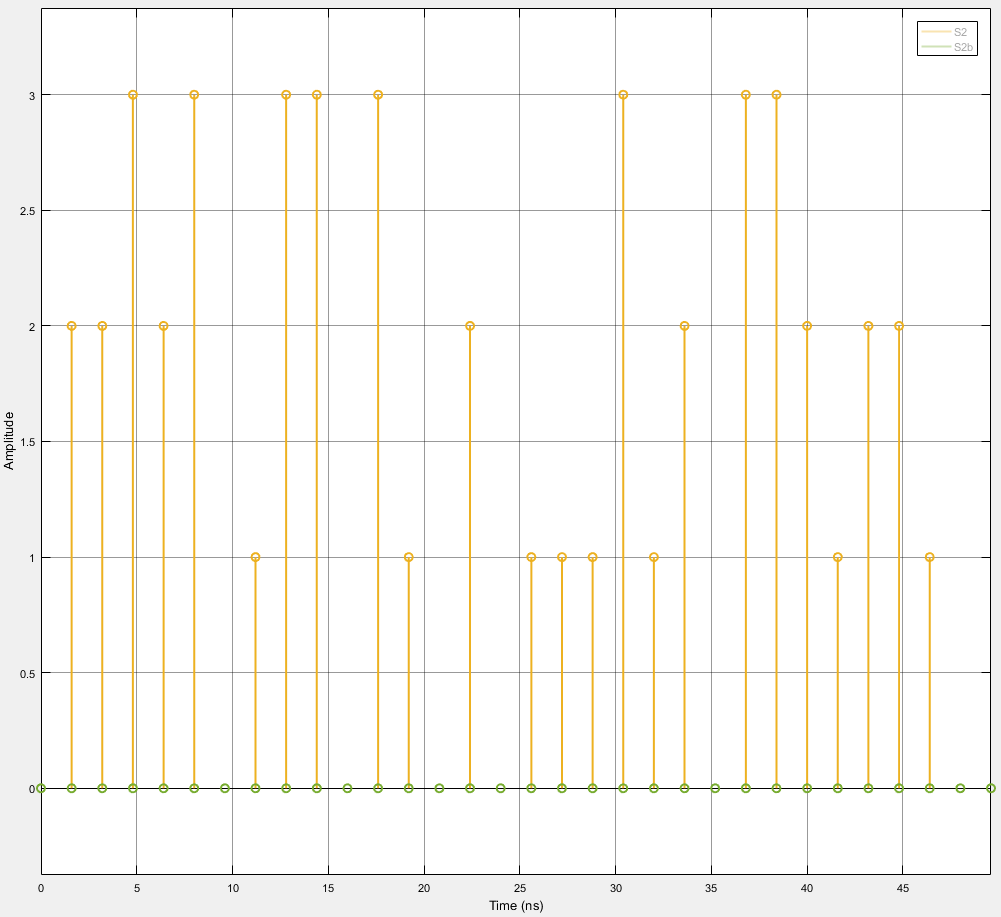
\includegraphics[width=0.9\textwidth, height=9cm]{./sdf/simplified_coherent_receiver/figures/S2S2b.png}
	\caption{S2 and S2b}\label{}
\end{figure}

\begin{figure}[h]
	\centering
	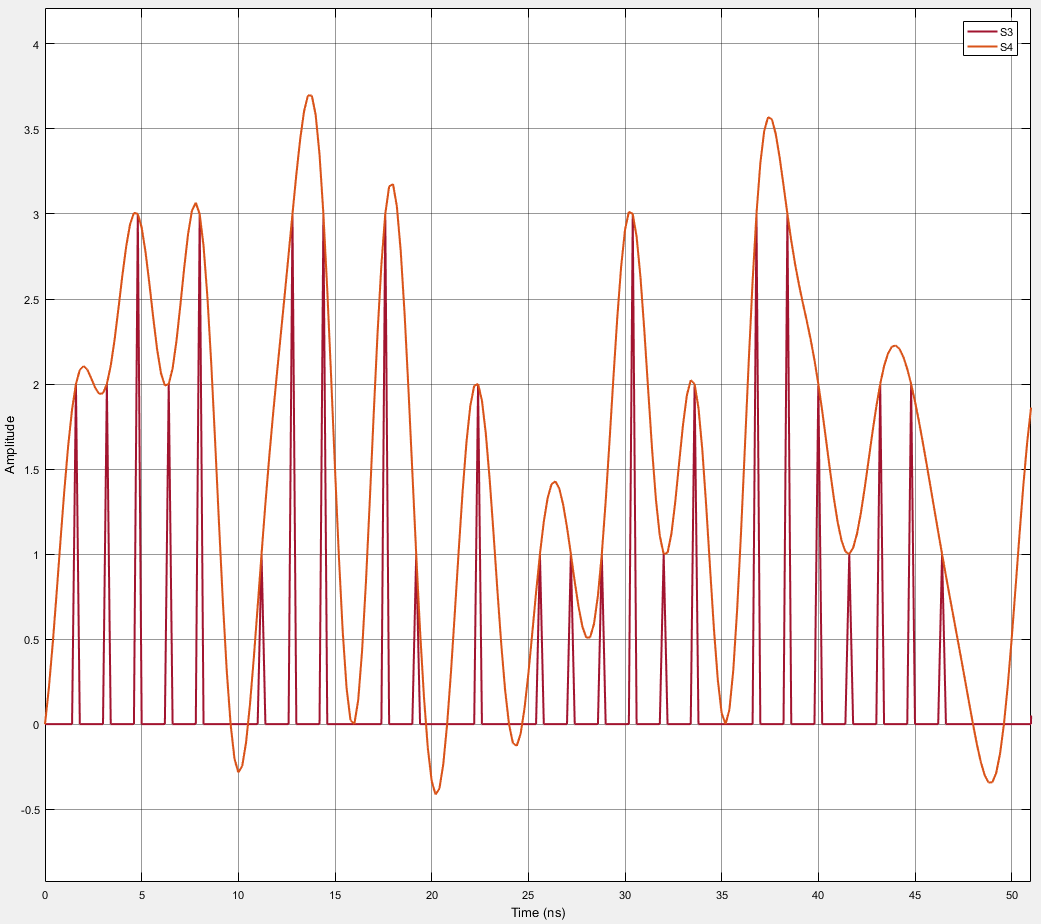
\includegraphics[width=0.9\textwidth, height=9cm]{./sdf/simplified_coherent_receiver/figures/S3S4.png}
	\caption{S3 and S4}\label{}
\end{figure}

\begin{figure}[h]
	\centering
	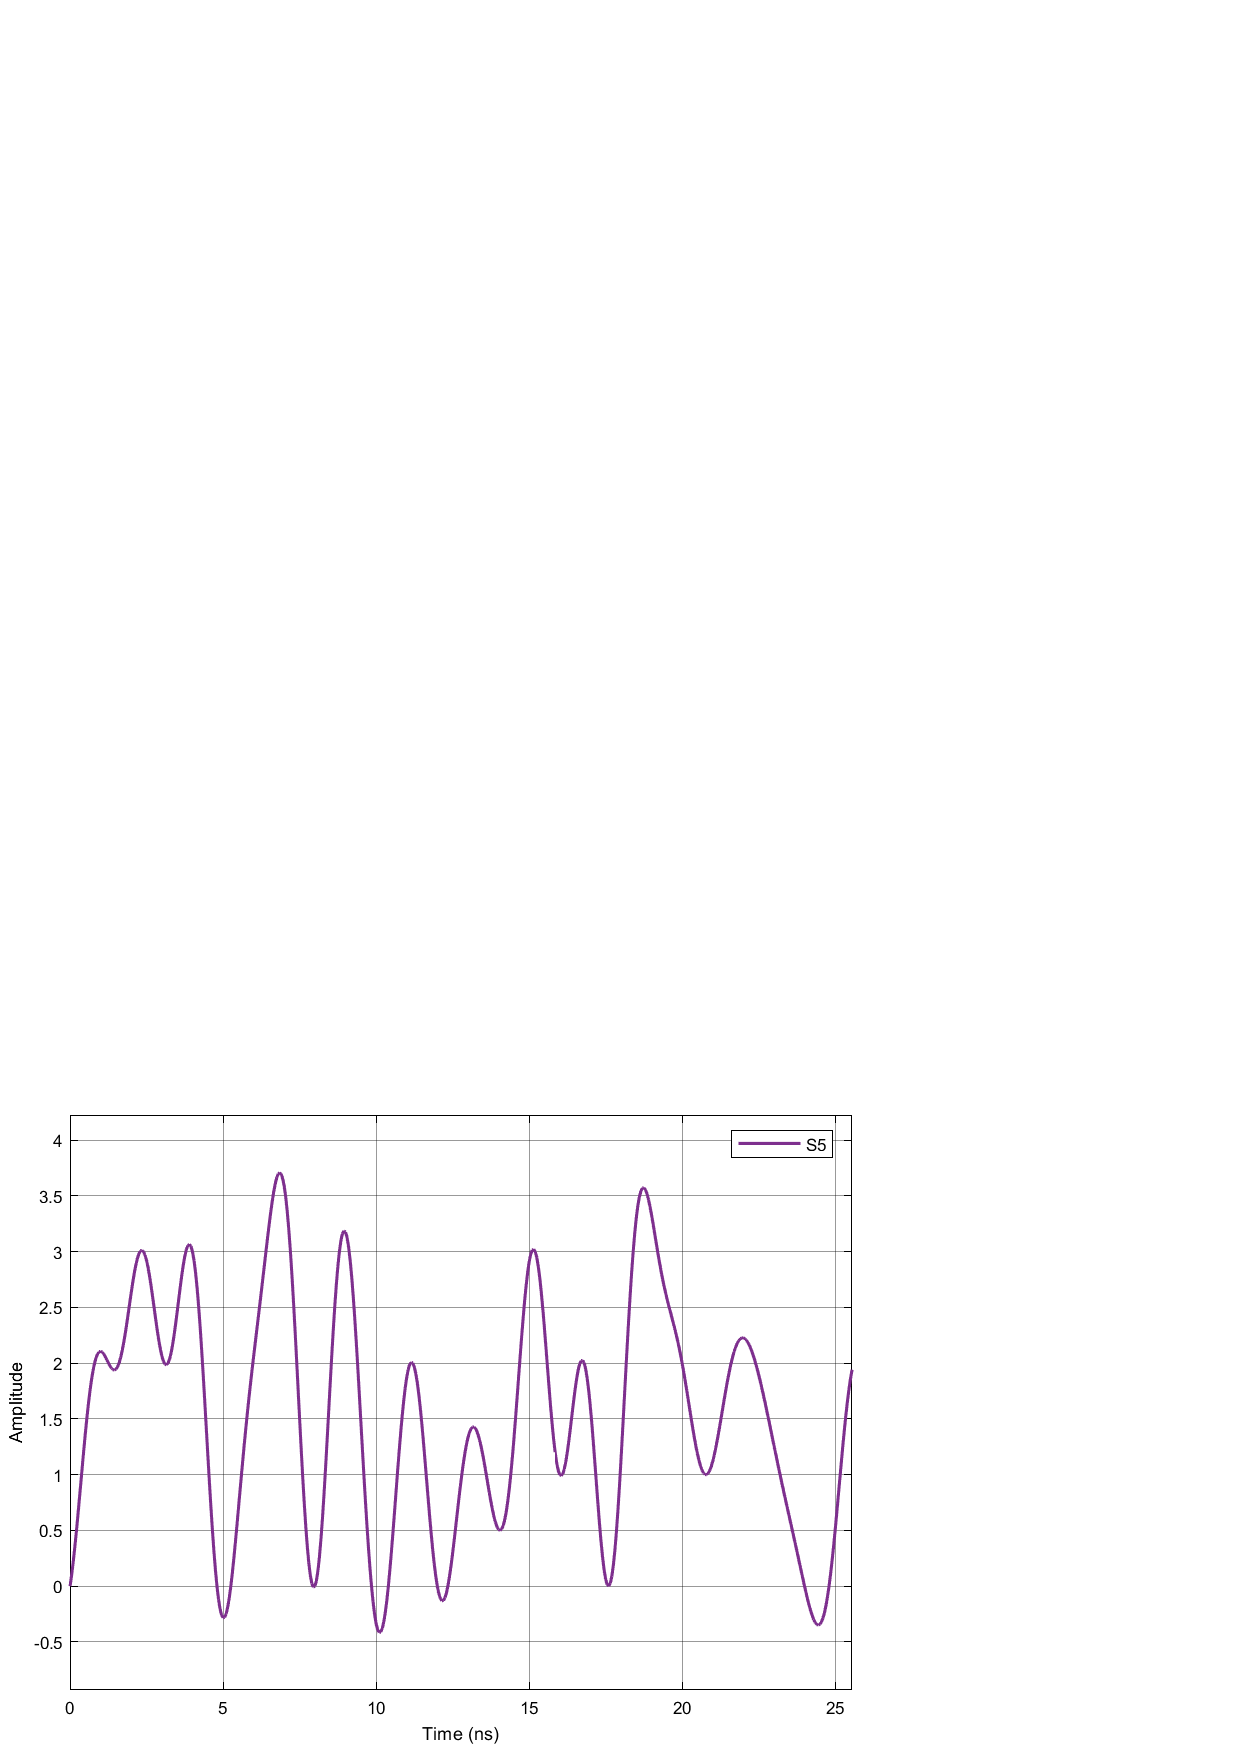
\includegraphics[width=0.9\textwidth, height=9cm]{./sdf/simplified_coherent_receiver/figures/S5.png}
	\caption{S5}\label{}
\end{figure}

\begin{figure}[h]
	\centering
	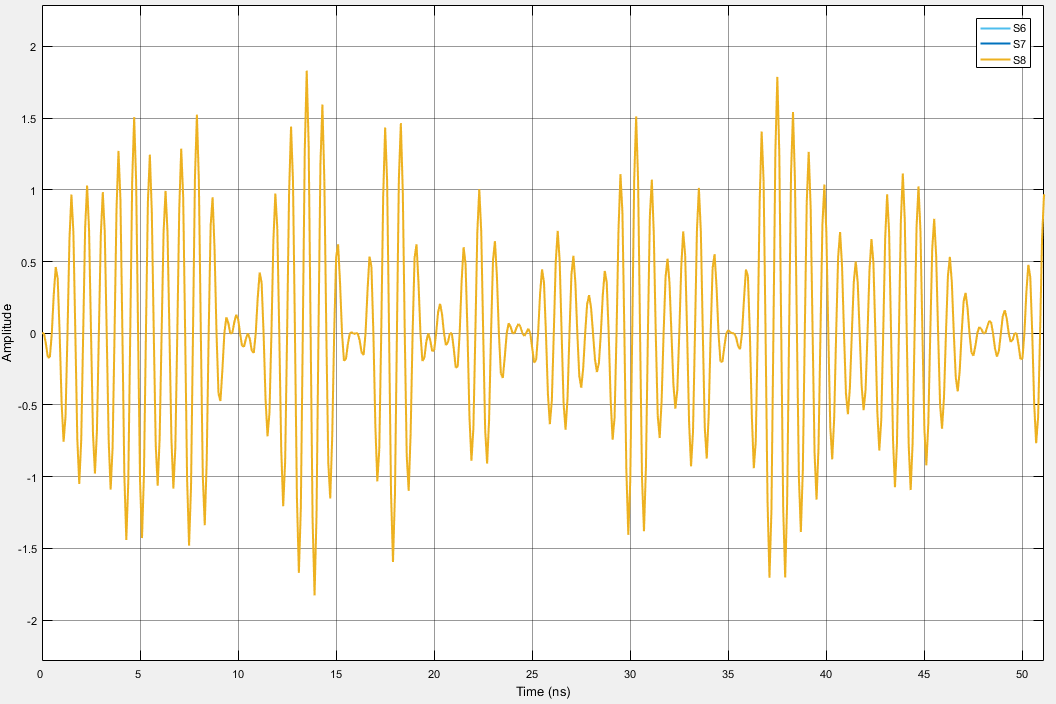
\includegraphics[width=0.9\textwidth, height=9cm]{./sdf/simplified_coherent_receiver/figures/S6S7S8.png}
	\caption{S6, S7 and S8}\label{}
\end{figure}

\begin{figure}[h]
	\centering
	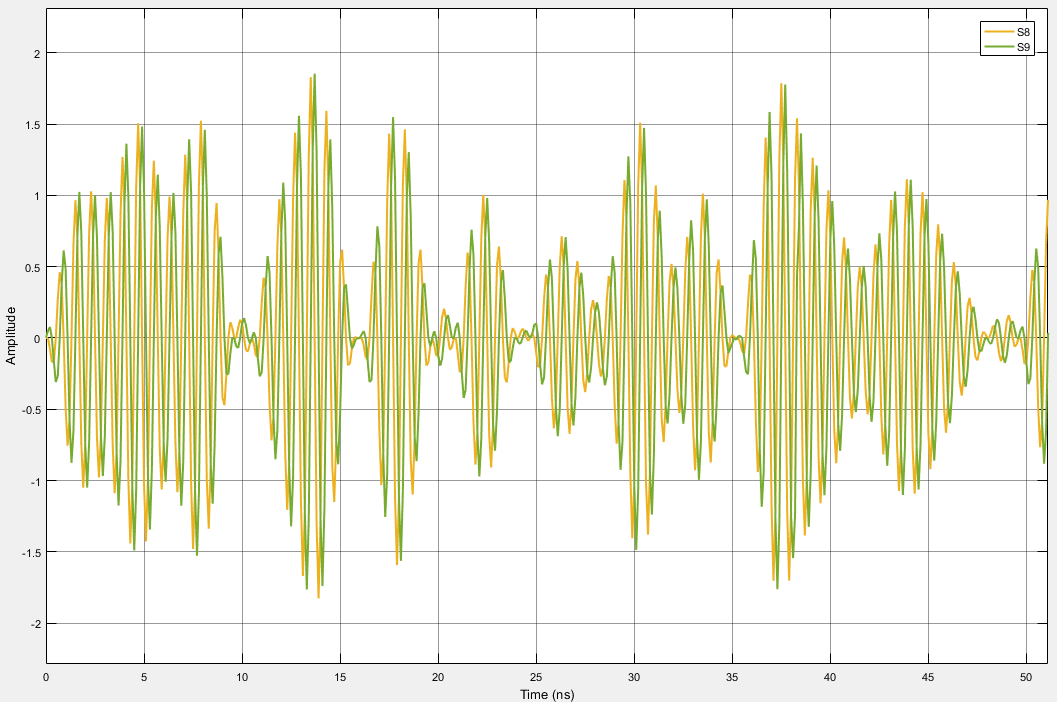
\includegraphics[width=0.9\textwidth, height=9cm]{./sdf/simplified_coherent_receiver/figures/S8S9.png}
	\caption{S8 and S9}\label{}
\end{figure}

\subsubsection{Receiver setup}
\begin{figure}[h]
	\centering
	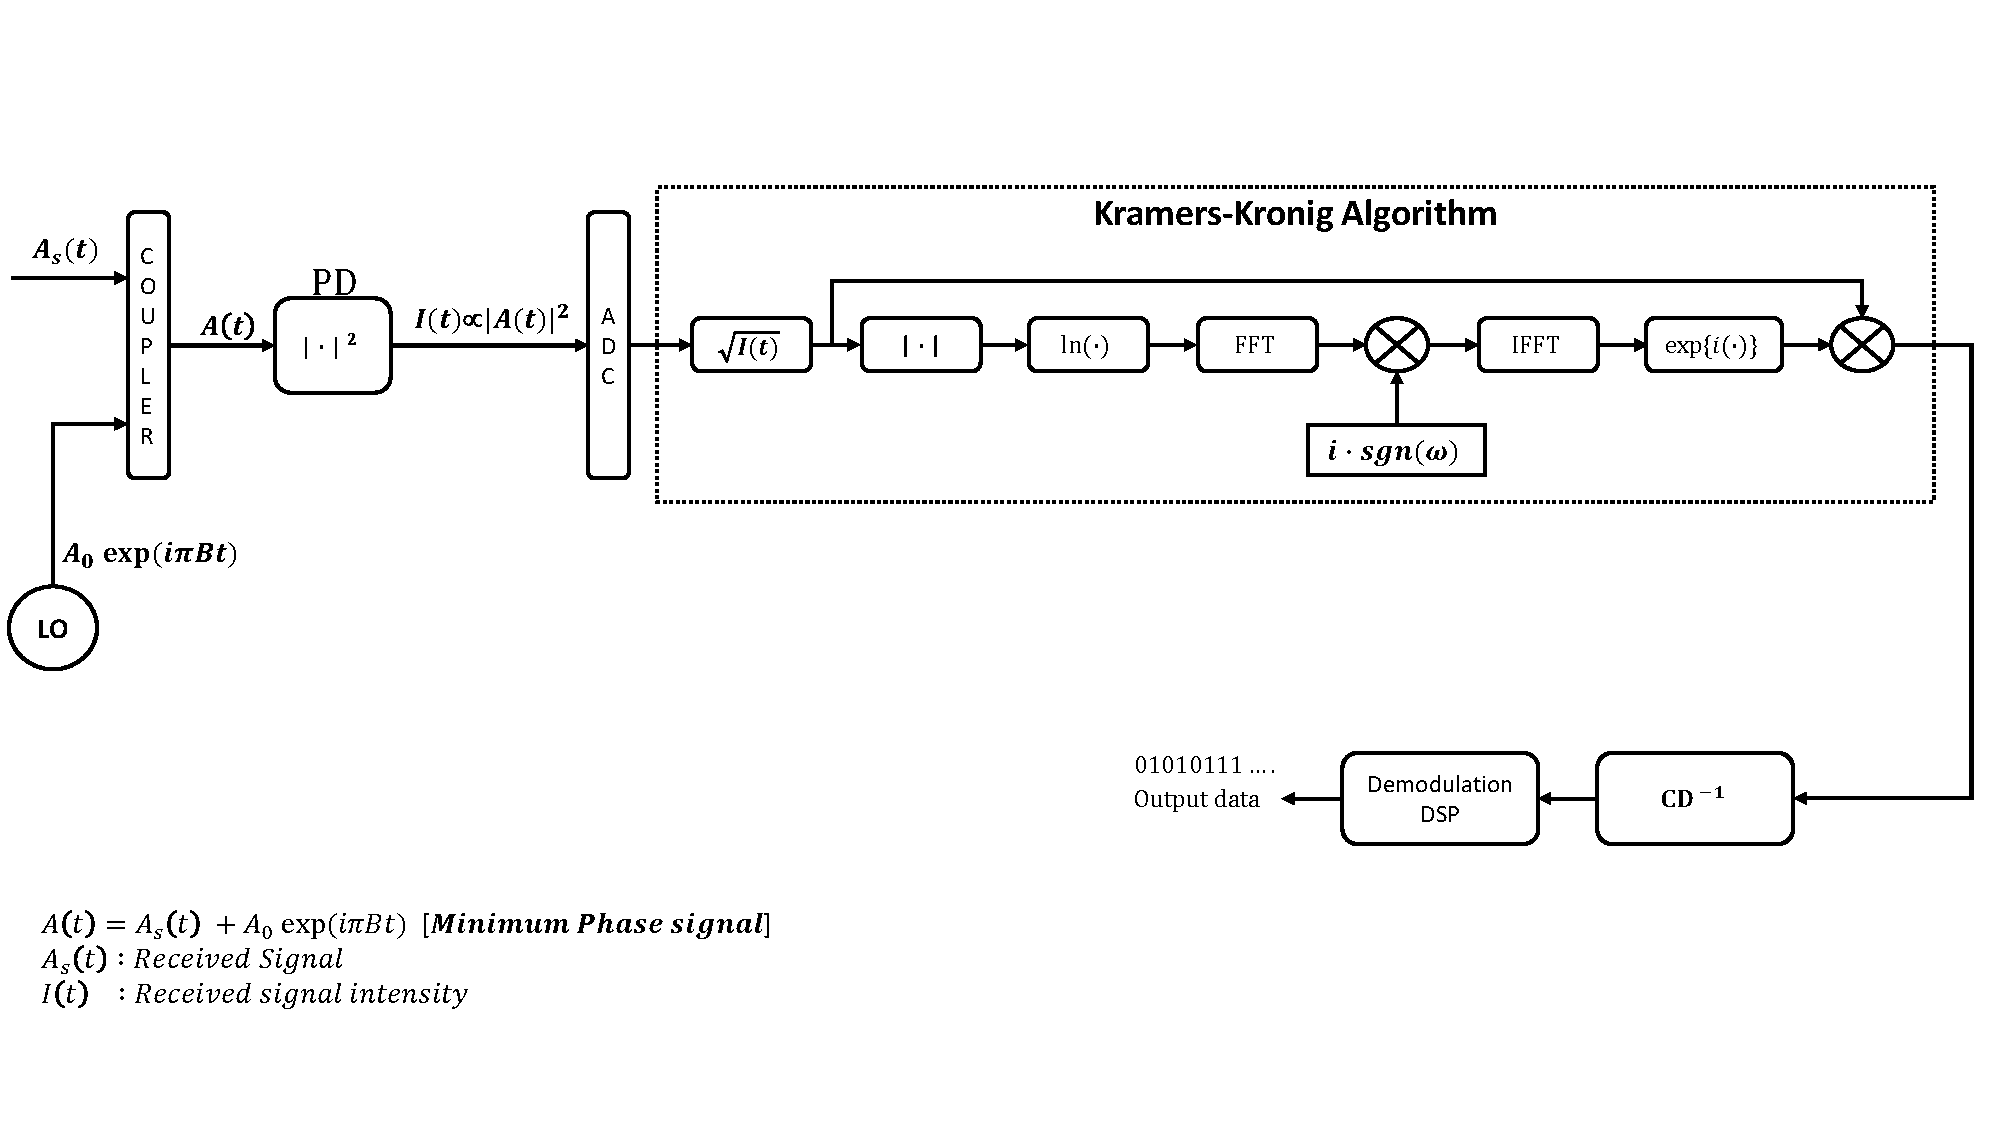
\includegraphics[width=1.0\textwidth, height=10cm]{./sdf/simplified_coherent_receiver/figures/Simulation_setup_Rx.pdf}
	\caption{Receiver simulation setup}\label{Simulation_setup_Rx}
\end{figure}
\newpage
\subsection{Experimental Analysis}
 As shown in the Figure \ref{Practical_setup_TxRx}, at the transmitter end, analytical signal generated with the help of netxpto and applied to the AWG. Waveform generated by AWG applied dual polarization IQ modulator which generates SSB signal in optical domain. SSB optical signal generated by both the IQ modulator is then combined using polarization beam combiner (PBC) and launched into the optical fiber.\\
 At the receiver end, the PDM received signal first spitted by a polarization beam splitter (PBS). Each polarization is combined with an LO tapped from the transmit laser. The laser's wavelength and power are set to ensure that the received signal should satisfy the minimum phase condition. After direct-detection, Kramers-Kronig algorithm is performed on each polarization separately to recover full complex signal. After compensation of the chromatic dispersion, stokes parameter based poldemux algrithm can be applied to recover PDM signals.     
\begin{figure}[h]
	\centering
	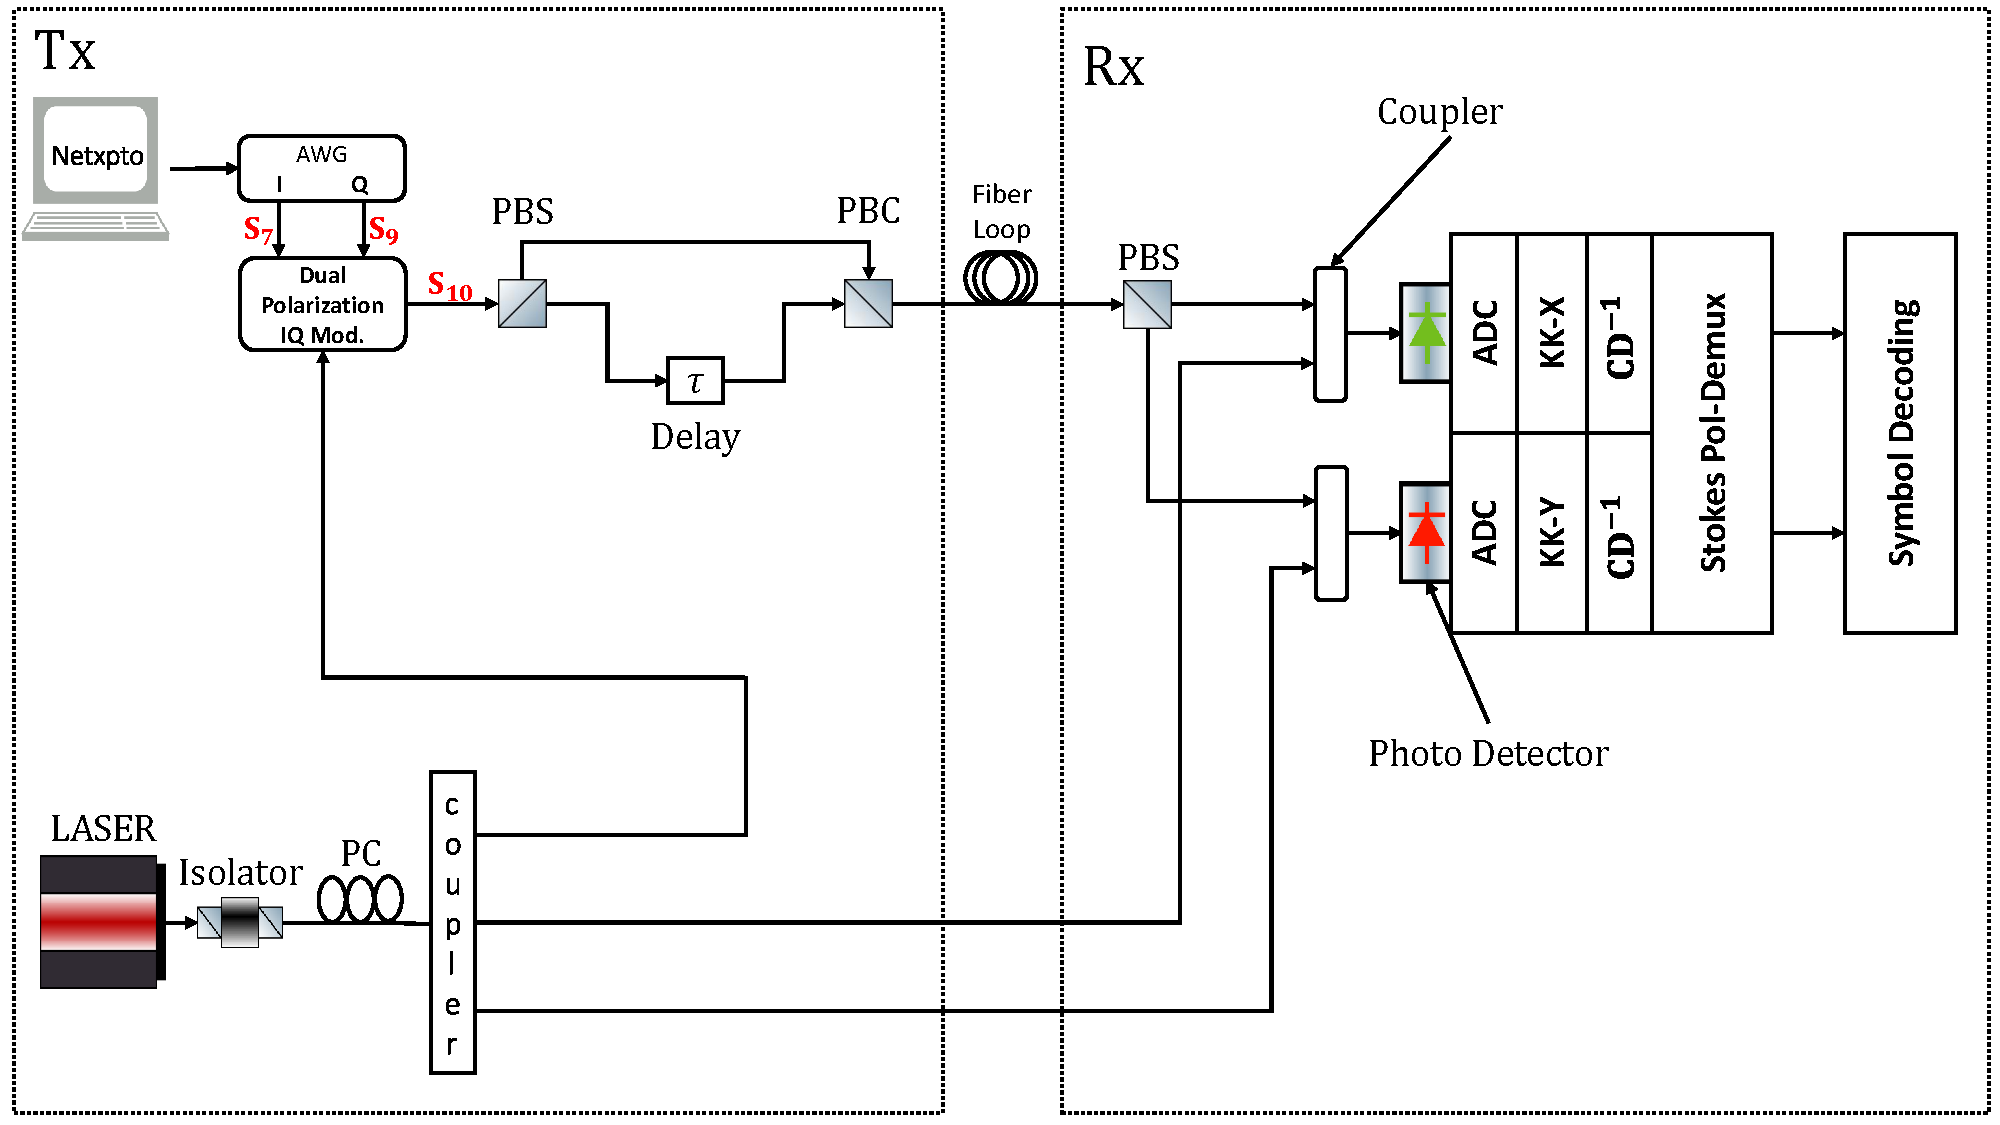
\includegraphics[width=1.0\textwidth, height=7cm]{./sdf/simplified_coherent_receiver/figures/Practical_setup_TxRx.pdf}
	\caption{PDM Kramers-Kronig receiver experimental setup}\label{Practical_setup_TxRx}
\end{figure}

\subsubsection{Status of equipment}
\begin{center}
	\begin{tabular}{ |p{6cm}||p{6.5cm}|p{1.5cm}|   }
		\hline
		%\multicolumn{3}{|c|}{\textbf{Source Files}} \\
		%\hline
		\textbf{Equipment name} & \textbf{Description}&\textbf{Status}\\
		\hline
		LASER				   				&  &\checkmark\\
		\hline
		PC	 								&  &\checkmark\\
		\hline
		Coupler							    &  &\checkmark\\
		\hline
		AWG									&  &\checkmark\\
		\hline
		Dual polarization IQ mod			&  &\checkmark\\
		\hline
		PBS				 					&  &\checkmark\\
		\hline
		PLC									&  &\checkmark\\
		\hline
		Delay								&  &\checkmark\\
		\hline
		Fiber loop							&  &\checkmark\\
		\hline
		Single photodetector				& APD+TIA Optical Receiver:\newline
											  - Maximum bit rate: 10 Gb/s\newline
											  - Sensitivity: -26 dBm &\checkmark\\
		\hline
	\end{tabular}
\end{center}

\subsection{Comparative Analysis}

\subsection{Know Problems}

\begin{center}
	\begin{tabular}{ |p{6cm}||p{6.5cm}|p{1.5cm}|   }
		\hline
		%\multicolumn{3}{|c|}{\textbf{Source Files}} \\
		%\hline
		\textbf{Problem type} & \textbf{Description}&\textbf{Note}\\
		\hline
		Simulator			& Require a generalized block for FFT and IFFT  &DONE!\\
		\hline
	\end{tabular}
\end{center}


\begin{thebibliography}{9}
	\bibitem{latexcompanion}
	Antonio Mecozzi, Cristian Antonelli, and Mark Shtaif.
	\textit{Kramers-Kronig Coherent Receiver}.
	Optica, vol.3, no.11, 2016, p.1220., doi:10.1364/optica.3.001220.
	
	\bibitem{latexcompanion}
	Antonio Mecozzi.
	\textit{Retrieving the full optical response from amplitude data by Hilbert transform}. Opt. Comm. 282, 4183-4187.
	
	\bibitem{latexcompanion}
	Antonio Mecozzi.
	\textit{A necessary and sufficient condition for minimum phase and implication of phase retrieval}. arXiv:1606.04861.
\end{thebibliography}

\subsubsection{\textbf{APPENDICES}}
%%%%%%%%%%%%%%%%%%%%%%%%%%%%%%%%%%%%%%%%%%%%%%%%%%%%%%%%%%%%%%%%%%%%%%%%%%%%%%%%%%%%%%%%%%%%%%%%%%%%%%%%%%
\textbf{Appendix A : SSB with graphical explanation}\\
This section describes the SSB signal generation using Hilbert transformation method (Phase Shift Method). Consider a message signal $m(t)$ with its frequency domain spectrum $M(F)$ as shown in Figure\ref{Original_baseband_signal}. From the Figure \ref{Original_baseband_signal}, we can see that both the side are scaled by factor '1' which means it represents the original signal.
\begin{figure}[h]
	\centering
	\includegraphics[width=0.6\textwidth, height=5cm]{./sdf/simplified_coherent_receiver/figures/SSB1.pdf}
	\caption{Original baseband signal}\label{Original_baseband_signal}
\end{figure}\\ 	
Now let's consider the modulated signal $x(t)$ given as,
\begin{equation}
x(t)=m(t) cos(2\pi f_c t)
\label{Eq:5.20}
\end{equation}
Frequency domain representation of the equation \ref{Eq:5.20} can be given as,
\begin{equation}
X(F)=\frac{1}{2}M(f-f_c)+\frac{1}{2}M(f+f_c)
\label{Eq:5.21}
\end{equation}
Here in equation \ref{Eq:5.21}, we can observe that each side band are scaled by $\dfrac{1}{2}$ on the frequency spectrum. Figure displays the frequency domain representation of the modulated signal $X(F)$.
\begin{figure}[h]
	\centering
	\includegraphics[width=1.0\textwidth, height=8cm]{./sdf/simplified_coherent_receiver/figures/SSB2.pdf}
	\caption{Original modulated signal}\label{Original_modulated_signal}
\end{figure}\\ 
Next, we will discuss something more interesting which is called as Hilbert transform of the original message signal $m(t)$. As we discussed earlier, in the frequency domain, the Hilbert transformed signal $\hat{M}(f)$ can be achieved by multiplying the Fourier transformed signal $M(F)$ with $[-i sgn(F)]$.
\begin{figure}[h]
	\centering
	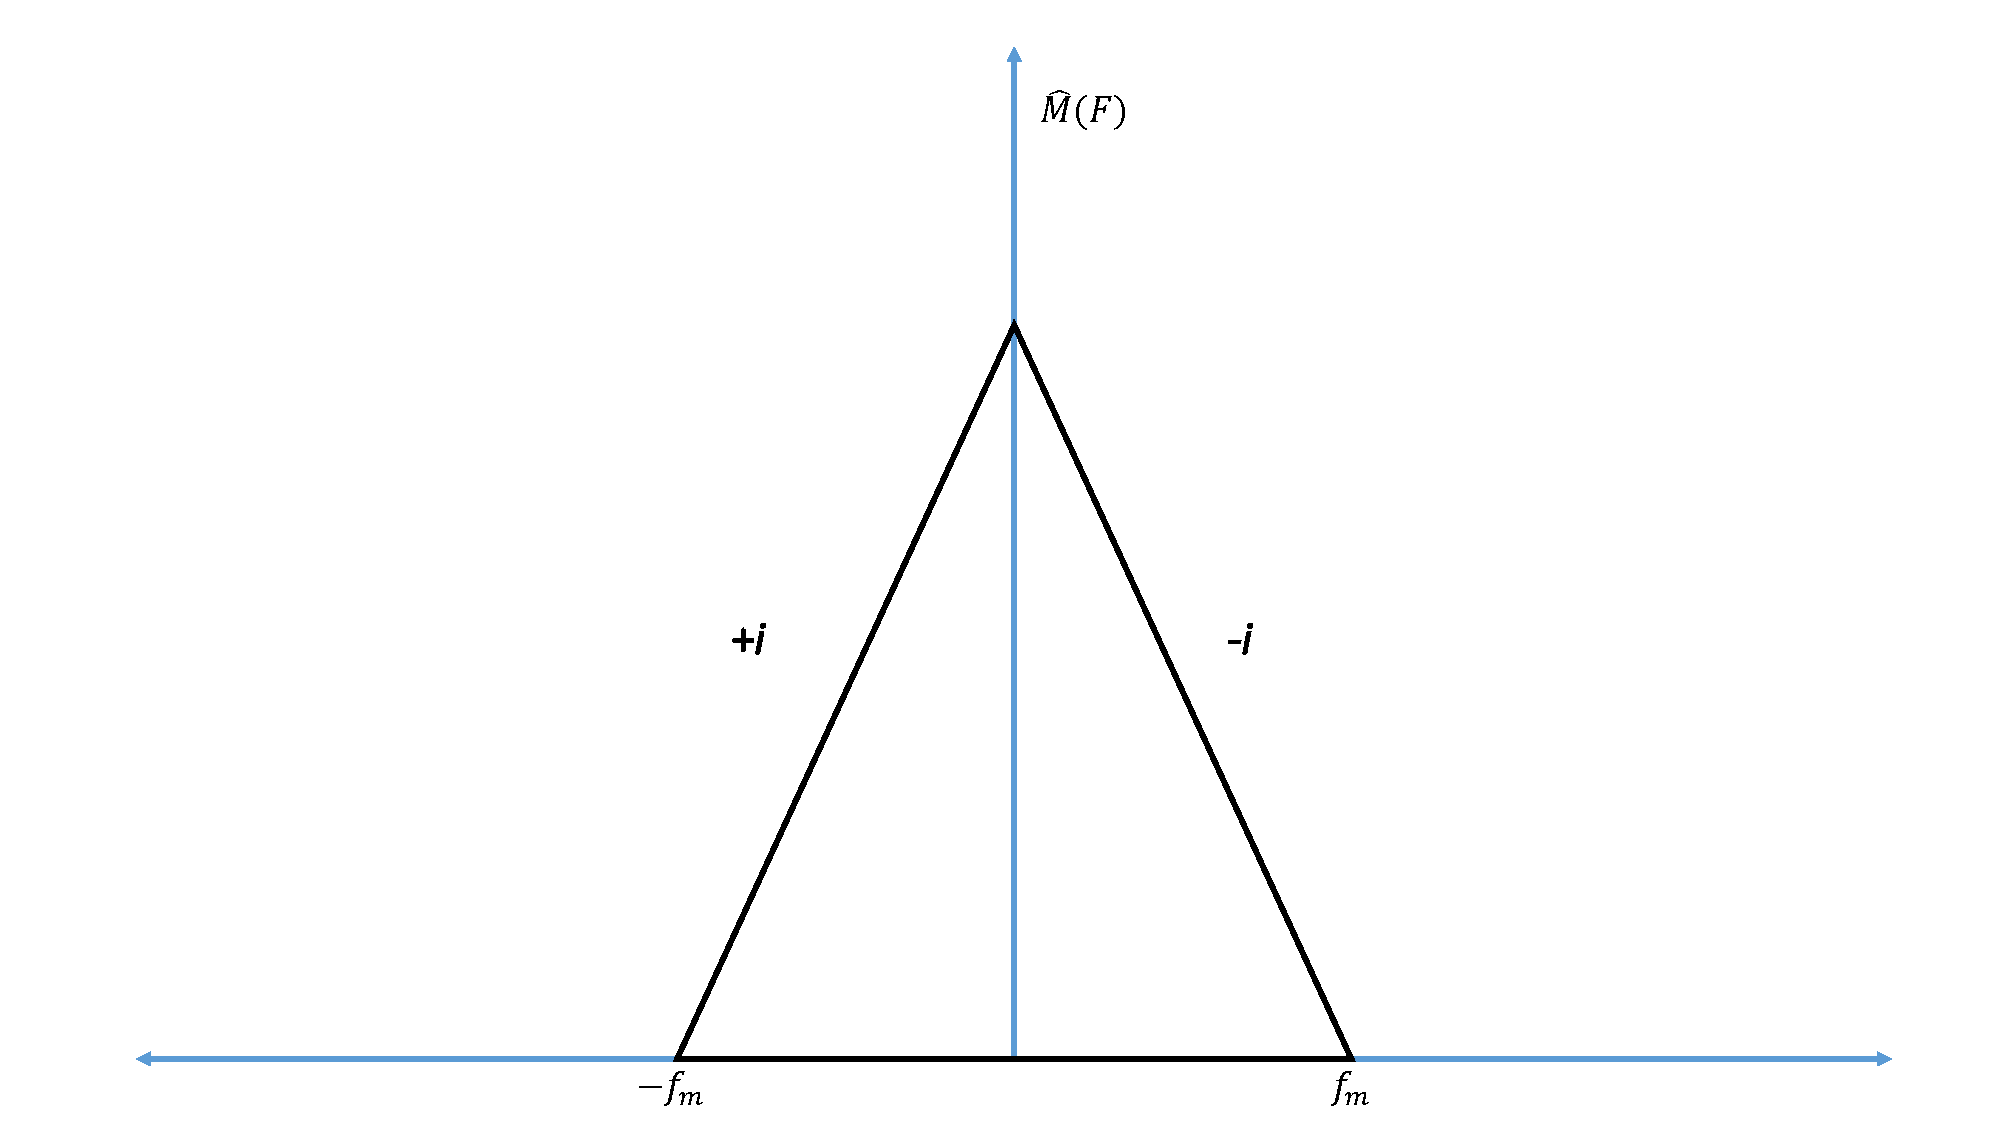
\includegraphics[width=0.6\textwidth, height=5cm]{./sdf/simplified_coherent_receiver/figures/SSB3.pdf}
	\caption{Hilbert transformed modulated signal}\label{Hilbert_Transformed_signal}
\end{figure}
Suppose we modulate the Hilbert transformed message signal $\hat{m}(t)$  with the $sin(2\pi f_c t)$ (quadrature phase carrier), then we get the following results:

\begin{equation}
\begin{split}
{\hat{m}(t)} sin(2\pi f_c t)&={\hat{m}(t)}\frac{e^{i2\pi f_c t} - e^{-i2\pi f_c t} }{2}\\
&={\hat{m}(t)}\frac{e^{i2\pi f_c t}}{2} - {\hat{m}(t)}\frac{e^{-i2\pi f_c t}}{2}\\
&={\frac{\hat{M}(f-f_c)}{2i}}-{\frac{\hat{M}(f+f_c)}{2i}}\\
&={\frac{-i}{2}\hat{M}(f-f_c)}+{\frac{-i}{2}\hat{M}(f+f_c)}\\
\end{split}
\label{Eq:5.46}
\end{equation}
The detailed explanation of the equation \ref{Eq:5.46} has been given in the Figure \ref{Hilbert_Transformed_modulated_signal} and \ref{Hilbert_Final}. Figure \ref{Hilbert_Transformed_modulated_signal} displays the spectrum of the $\hat{M}(f+f_c)$ and $\hat{M}(f-f_c)$ for the positive and negative frequencies respectively. The final equation resolution of equation displays that both positive and negative side of the spectrum multiplied with $\frac{i}{2}$ and $\frac{-i}{2}$ respectively. Finally the spectrum of the signal ${\hat{m}(t)} sin(2\pi f_c t)$ can be given as Figure \ref{Hilbert_Final}.
\begin{figure}[h]
	\centering
	\includegraphics[width=1.0\textwidth, height=8cm]{./sdf/simplified_coherent_receiver/figures/SSB4.pdf}
	\caption{Hilbert transformed modulated signal}\label{Hilbert_Transformed_modulated_signal}
\end{figure}

\begin{figure}[h]
	\centering
	\includegraphics[width=1.0\textwidth, height=8cm]{./sdf/simplified_coherent_receiver/figures/SSB5.pdf}
	\caption{Hilbert transformed modulated signal}\label{Hilbert_Final}
\end{figure}

Further, summation of the two signals ${m(t)} cos(2\pi f_c t)$ and ${\hat{m}(t)} sin(2\pi f_c t)$ will generate the upper sideband SSB signal as follows,
\begin{equation}
u(t)={m(t)} cos(2\pi f_c t)-{\hat{m}(t)} sin(2\pi f_c t)
\label{5.23}
\end{equation}
From the above discussion, the spectrum of the Equation \ref{5.23} can be given by the Figure \ref{SSB_signal_spectrum}. Similarly, for the lower sideband SSB can be generated by Equation,
\begin{equation}
u(t)={m(t)} cos(2\pi f_c t)+{\hat{m}(t)} sin(2\pi f_c t)
\label{5.24}
\end{equation}
\begin{figure}[h]
	\centering
	\includegraphics[width=1.0\textwidth, height=8cm]{./sdf/simplified_coherent_receiver/figures/SSB6.pdf}
	\caption{SSB signal spectrum}\label{SSB_signal_spectrum}
\end{figure}
%%%%%%%%%%%%%%%%%%%%%%%%%%%%%%%%%%%%%%%%%%%%%%%%%%%%%%%%%%%%%%%%%%%%%%%%%%%%%%%%%%%%%%%%%%%%%%%%%%%%%%%%%%
\textbf{Appendix B : Kramers-Kronig scheme}\\
If we consider the complex envelope of the incoming electric field by $A_s(t)$ confined within the optical bandwidth denoted by B. The LO assumed to be a continuous wave (CW) signal whose amplitude is $A_0$ whose frequency coincides with the left edge of the information-carrying signal spectrum. Here, we assumed that $A_0$ is real-valued and positive, which is equivalent to referring all phase value to that of LO.\\
The complex envelope of the field striking upon the photo-diode can be given as,
\begin{equation}
A(t)=A_s(t)+A_0 exp(i\pi Bt)
\end{equation}
The photo current $I$ produced by the photo-diode is proportional to the field intensity $I=|A(t)|^2$, here proportionality constant considered as 1 for the sake of simplicity. If $A_0$ is large enough to ensure that the signal $A(t)exp(-i\pi Bt)=A_0+A_s(t)exp(-i\pi Bt)$ is minimum phase. The discussed hypothesis can be used to reconstruct the signal $E_s(t)$ as follows[1]:
\begin{equation}
A_s(t)=\{\sqrt{I(t)} exp[i\phi_E(t)]-A_0\} exp(i\pi Bt)
\end{equation}
\begin{equation}
\phi_A(t)=\dfrac{1}{2\pi} p.v. \int_{-\infty}^{\infty} dt' \frac{log[|I(t')|]}{t-t'}
\label{Eq:5.19}
\end{equation}
